\documentclass[11pt]{article}
\newcommand{\name}{Jingbo Wang}

\usepackage[paper=letterpaper, margin=1in, headheight=13.6pt]{geometry}
\usepackage{fancyhdr}
\pagestyle{fancy}
\fancyhf{}
\rhead{\name{}}
\cfoot{Page \thepage}

\usepackage[parfill]{parskip}
\usepackage{amsmath}
\usepackage{graphicx}
\usepackage{fancyvrb}
\usepackage{upquote}

\begin{document}
\thispagestyle{empty}

\begin{center}
{\large CS 310}\\
Assignment 202\\
\today
\end{center}

\begin{flushright}
\name{}
\end{flushright}

The \texttt{foo} algorithm given in the assignment could could sort the
randomly created vector which size is decided by user.
This is accomplished by \texttt{foo} function.

The input size of the \texttt{foo} algorithm is n, defined on line 3 of 
the program.  

This algorithm has distinct best and worst cases. The best case
occurs when line 18 always is false when running every times. In other 
words, it means this random numbers are already in ordered.
Therefore, We have:
\begin{itemize}
 \item Line 03: one assignment n for the size of vector: 1 operation
 \item Line 05: the outer for loop runs twice for hear every times  
                  and runs $n - 1$ times, and total operation: 
                  $2(n-1) + 2 = 2n$ operations
 \item Line 07: one assignment item to get the value of start 
                  position's value, two operation for each: 
                  $\times (n - 1)$ times: $2 \times (n - 1) = 2n - 2$
                  operations.
 \item Line 08: one assignment position to get the position of start 
                  position$\times (n - 1)$ times: $1 \times (n - 1) 
                  = n - 1$ operations.
 \item Line 10: the inner for loop runs twice for hear every times  
                  and runs n times, and $n - 1$ last time,and 2 
                  operations each,so the total operations: 
                  $2\frac{n((n-1) + 0)}{2} + 2(n - 1)= n^{2} + n - 2$
                  operations.
 \item Line 12: the if statement in the inner for loop always is 
                  false, two operations for each. It runs $n-1$ 
                  times. We can get: $2\frac{n((n-1) + 0)}{2} = 
                  n^{2} - n$ operations.
 \item Line 18: the next if statement in the outer for loop is false, 
                  one operation for each. It runs $n - 1$ times. 
                  We can get: $1 \times (n - 1) = n - 1$ operations.
\end{itemize}
So, we can get the total operations for best case is $1 + 2n + 
    (n - 1) + (2n - 2)+ (n^{2} + n - 2) + (n^{2} - n) + (n - 1)
    = 2n^{2} + 6n - 5$  

Also, the worst case occurs when the if statements and while loops 
always are true when running every times.Therefore, We have:
\begin{itemize}
 \item Line 03: one assignment n for the size of vector: 1 operation
 \item Line 05: the outer for loop runs twice for hear every times  
                  and runs $n - 1$ times, and total operation: 
                  $2(n-1) + 2 = 2n$ operations
 \item Line 07: one assignment item to get the value of start 
                  position's value, two operation for each: 
                  $\times (n - 1)$ times: $2 \times (n - 1) = 2n - 2$
                  operations.
 \item Line 08: one assignment position to get the position of start 
                  position$\times (n - 1)$ times: $1 \times (n - 1) 
                  = n - 1$ operations.
 \item Line 10: the inner for loop runs twice for hear every times  
                  and runs $n - 1$ times, last time gets out,and 2 
                  operations each,so the total operations: 
                  $2\frac{n((n-1) + 0)}{2} + 2(n - 1)= n^{2} + n - 2$
                  operations.
 \item Line 12: the if statement in the inner for loop always is 
                  true, two operations for each. It runs $n-1$ 
                  times. We can get: $2\frac{n((n-1) + 0)}{2} = 
                  n^{2} - n$ operations.
 \item Line 14: position always plus one, one operation for each, 
                  run $n - 1$ time.so, the total operations are: 
                  $\frac{n((n - 1) + 0)}{2} = \frac{1}{2}n^{2}-
                  \frac{1}{2}n$ operations.
 \item Line 18: the next if statement in the outer for loop is always  
                  true, one operation for each. It runs $n - 1$ times. 
                  We can get: $1 \times (n - 1) = n - 1$ operations.
 \item Line 20:  the while loop runs each times in the outer for loop, 
                   run $n-1$ times, two operations for each, so the 
                   total operations is: $2\frac{n((n-1) + 0)}{2} 
                   + 2(n - 1) = n^{2} + n - 2$ operations. 
 \item Line 22:  position always plus one, one operation for each, 
                   run $n - 1$ time in the while loop.
                   so, the total operations are: $\frac{n((n - 1) + 
                  0)}{2} = \frac{1}{2}n^{2}-\frac{1}{2}n$ operations.
 \item Line 24:  the swap function is always called after the first
                   while loop for $n - 1$ times,two operations for
                   each. The total operations are: $2(n - 1)
                   = 2n - 2$ operations.
  \item Line 26: the while loop runs each times in the outer for loop, 
                   run $n-1$ times, one operations for each, so the 
                   total operations is: $\frac{n((n-1) + 0)}{2} 
                   + (n - 1)= \frac{1}{2}n^{2} + \frac{1}{2}n - 1$ 
                   operations.
  \item Line 28: one assignment position to get start position, 
                   run $n - 2$ time in the while loop, one operation 
                   for each. So, the total operations are: 
                   $\frac{n((n - 1) + 0)}{2} = \frac{1}{2}n^{2}-
                   \frac{1}{2}n$ operations.
  \item Line 29: the inner for loop in the while loop, and $n - 1$ 
                  last time,and 2 operations each,so the total 
                  operations: $2\frac{n((n-1) + 0)}{2} + 2(n - 1)
                  = n^{2} + n - 2$ operations.
  \item Line 31: the if statement in the inner for loop always is 
                  true, two operations for each. It runs $n-1$ 
                  times. We can get: $2\frac{n((n-1) + 0)}{2} = 
                  n^{2} - n$ operations.
  \item Line 33: position always plus one, runs $n - 1$ time.so,
                  one operation for each,the total operations are: 
                  $\frac{n((n - 1) + 0)}{2} = \frac{1}{2}n^{2} -
                  \frac{1}{2}n$ operations.
  \item Line 37: the inner while loop in the while loop runs $n - 1$ 
                   time, one operation for each. The total operations 
                  are: $2\frac{n(0 + (n - 1))}{2}+2(n - 1) = n^{2}
                  + n - 2$ operations.
  \item Line 39: position always plus one, runs $n - 1$ time.so,
                  one operation for each,the total operations are: 
                  $\frac{n((n - 1) + 0)}{2} = \frac{1}{2}n^{2} -
                  \frac{1}{2}n$ operations. 
  \item Line 41: the swap function is always called after the first
                   while loop for $n - 1$ times, two operations for
                   each. The total operations are: $2(n - 1)
                   = 2n - 2$ operations.
\end{itemize}
So, we can get the total operations for worst case is 
     $1  
      + (2n) 
      + (2n - 2) 
      + (n - 1) 
      + (n^{2} + n - 2) 
      + (n^{2} - n) 
      + (\frac{1}{2}n^{2} - \frac{1}{2}n) 
      + (n - 1) 
      + (n^{2} + n - 2) 
      + (\frac{1}{2}n^{2} - \frac{1}{2}n) 
      + (2n -2) 
      + (\frac{1}{2}n^{2} + \frac{1}{2}n - 1)
      + (\frac{1}{2}n^{2} - \frac{1}{2}n)
      + (n^{2} + n - 2)
      + (n^{2} - n)
      + (\frac{1}{2}n^{2} - \frac{1}{2}n) 
      + (n^{2} + n - 2)
      + (\frac{1}{2}n^{2} - \frac{1}{2}n)
      + (2n -2) = 9n^{2} + 10n - 16$

Therefore we conclude that the efficiency of this algorithm is

\begin{align*}
  T(n) \leq 9n^{2} + 10n - 16 &\in O(n^{2})\\
       \geq 2n^{2} + 6n - 5 &\in \Omega(n^{2})
\end{align*}

or equivalently,

\[
T(n) \in \Theta(n^2)
\]

In order to visualize this analysis, the program was annotated with
counters.  See the attached code, with comments indicating where the
counts occur.  The program was run with the command

\begin{Verbatim}
for n in $(seq 100 10 10000)
do
    ./program $n
    ./program $n
    ./program $n
done 2> results.dat
\end{Verbatim}

in order to generate a set of points.  The resulting data were
plotted, giving the following.  Also plotted on the same axes are the
scaled standard functions $9n^{2} + 10n - 1$ and $2n^{2} + 6n - 5$ 
which illustrate that $9n^{2} + 10n - 1$ that above the algorithm is 
worst case, and $2n^{2} + 6n - 5$ below the algorithm is the best 
case.

\begin{center}
  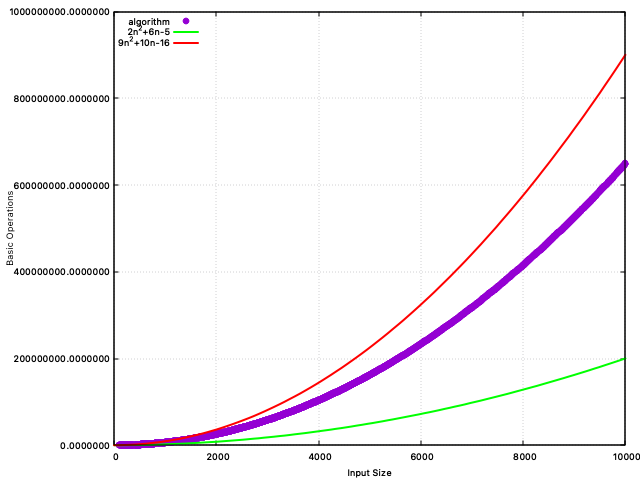
\includegraphics[width=0.7\textwidth]{analysis}
\end{center} 

We see that the plot confirms the theoretical analysis above.

\end{document}